\documentclass[tikz,border=5mm]{standalone}
\usepackage{tikz}
\usetikzlibrary{arrows.meta, positioning, shapes.geometric, calc, backgrounds, fit, matrix, patterns, decorations.pathmorphing, decorations.markings, shadows}

% --- COLOR DEFINITIONS ---
\definecolor{Garnet}{HTML}{73000A}
\definecolor{CSecondaryRed}{HTML}{CC2E40}
\definecolor{CBlue}{HTML}{466A9F}
\definecolor{CDark}{HTML}{1F414D}
\definecolor{COlive}{HTML}{65780B}
\definecolor{CLime}{HTML}{CED318}
\definecolor{CGold}{HTML}{A49137}
\definecolor{CGrayLight}{HTML}{E5E5E5}
\definecolor{CGrayDark}{HTML}{555555}
\definecolor{CWhite}{HTML}{FFFFFF}

\begin{document}

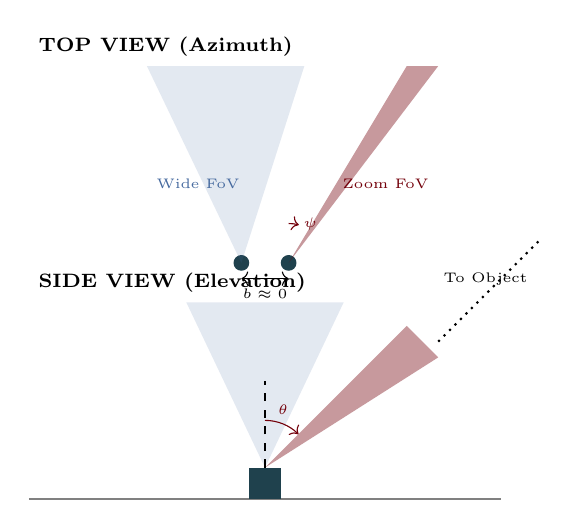
\begin{tikzpicture}
    % --- TOP VIEW (Azimuth) ---
    \begin{scope}[yshift=2cm]
        \node[font=\bfseries\scriptsize, anchor=south west] at (-3, 2.5) {TOP VIEW (Azimuth)};
        \coordinate (TC1) at (-0.3, 0);
        \coordinate (TC2) at (0.3, 0);
        
        \fill[CDark] (TC1) circle (0.1);
        \fill[CDark] (TC2) circle (0.1);
        \draw[<->] (-0.3, -0.2) -- (0.3, -0.2) node[midway, below, font=\tiny] {$b \approx 0$};
        
        % Beams
        \fill[CBlue, opacity=0.15] (TC1) -- (-1.5, 2.5) -- (0.5, 2.5) -- cycle; % Wide
        \fill[Garnet, opacity=0.4] (TC2) -- (1.8, 2.5) -- (2.2, 2.5) -- cycle; % Zoom
        
        % Angles
        \draw[->, Garnet] (TC2)++(0, 0.5) arc (90:75:0.5) node[midway, right, font=\tiny] {$\psi$};
        
        \node[right, font=\tiny, CBlue] at (-1.5, 1) {Wide FoV};
        \node[left, font=\tiny, Garnet] at (2.2, 1) {Zoom FoV};
    \end{scope}

    % --- SIDE VIEW (Elevation) ---
    \begin{scope}[yshift=-1cm]
        \node[font=\bfseries\scriptsize, anchor=south west] at (-3, 2.5) {SIDE VIEW (Elevation)};
        % Ground
        \draw[thick, gray] (-3, 0) -- (3, 0);
        \fill[CDark] (-0.2, 0) rectangle (0.2, 0.4); % Tripod head
        \coordinate (SC) at (0, 0.4);
        
        % Wide Vertical FoV
        \fill[CBlue, opacity=0.15] (SC) -- (-1, 2.5) -- (1, 2.5) -- cycle;
        
        % Zoom Vertical FoV (Tilted Up)
        \fill[Garnet, opacity=0.4] (SC) -- (1.8, 2.2) -- (2.2, 1.8) -- cycle;
        
        % Tilt Angle
        \draw[dashed] (SC) -- (0, 1.5); % Zenith/Normal
        \draw[->, Garnet] (0, 1.0) arc (90:45:0.6) node[midway, above, font=\tiny] {$\theta$};
        
        % Distant Object Representation
        \draw[dotted, thick] (2.2, 2.0) -- (3.5, 3.3);
        \node[font=\tiny] at (2.8, 2.8) {To Object};
    \end{scope}
\end{tikzpicture}

\end{document}
